\documentclass[UTF8]{ctexart}
\usepackage{datetime}
\usepackage{geometry}
\usepackage{array}
\usepackage{graphicx}
% 封面
\geometry{a4paper,left=1cm,right=2cm,top=1cm,bottom=1cm}
\title{\Huge xxxxxx}
\author{\Large 实验报告}
\begin{document}
\maketitle
\vspace{6\baselineskip}
\renewcommand\arraystretch{1.5}
\begin{table}[h]
      \centering
      \Large
      \setlength{\tabcolsep}{5mm}{
            \begin{tabular}{rcrc}
                  课程名称: & 数字电子技术 & 实验项目: & 集成触发器功能测试 \\

                  姓名:     & xxx       & 学号:     & xxxxxxxxx          \\

                  班级:     & xxxxxx      & 日期:     & \today             \\

                  地点:     & xxxx         & 成绩:     &                    \\
            \end{tabular}}
\end{table}

\vspace{10\baselineskip}

\centering
xxxxxxxx \\
\newpage


% 内容页
\begin{enumerate}
      \large
      \vspace{1\baselineskip}
      \item 原理及设计方案:  \\
            \begin{itemize}
                  \item [1.] 基本RS触发器(去抖) \\
                        \begin{center}  
                              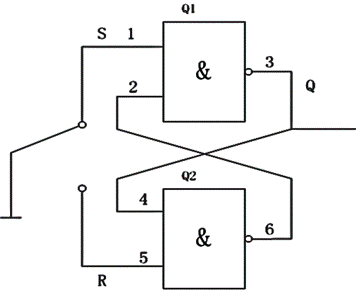
\includegraphics[scale=0.6]{1.png}
                              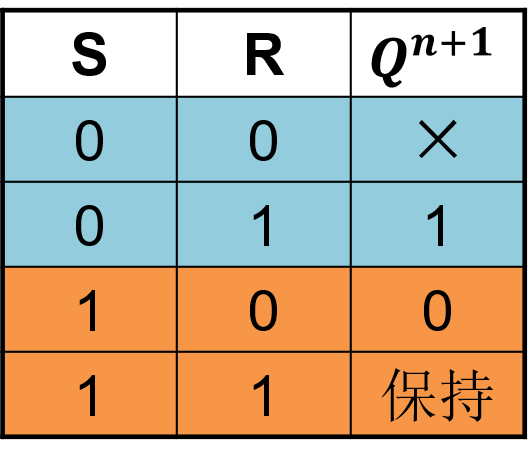
\includegraphics[scale=0.6]{2.png}
                        \end{center}

                  \item [2.] JK触发器 \\
                        \begin{center}
                              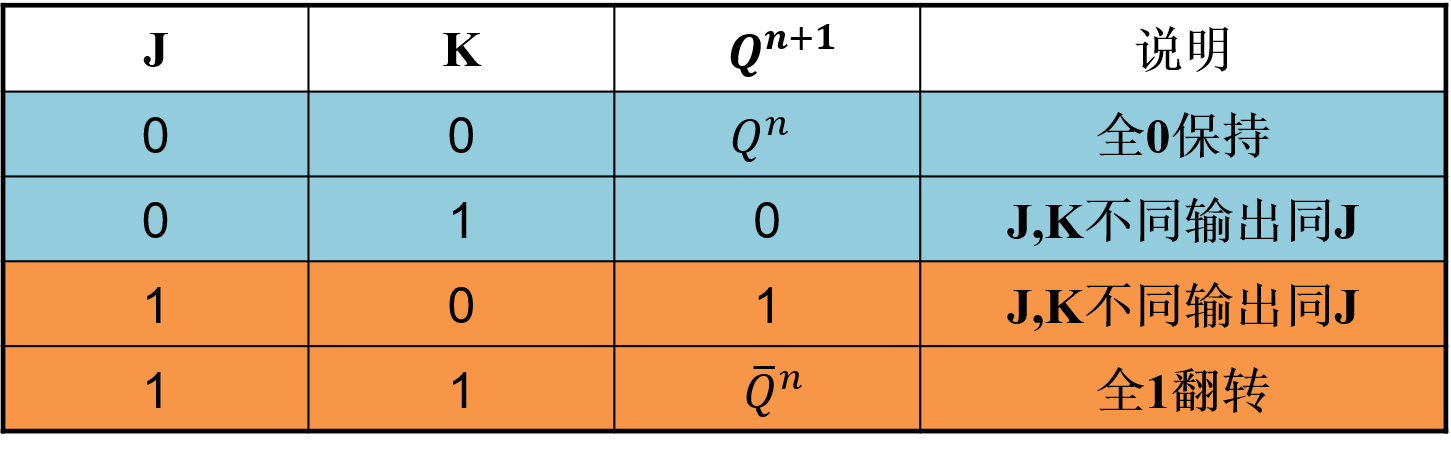
\includegraphics[scale = 0.6]{3.png}
                        \end{center}

                        \begin{itemize}
                              \item $\overline{RD},\overline{SD}$的复位,置零功能
                              \item $JK$ 输入端
                              \item $\overline{CP}$ 时钟端
                              \item $Q$,$\overline{Q}$ 输出端
                        \end{itemize}
                        \begin{center}
                              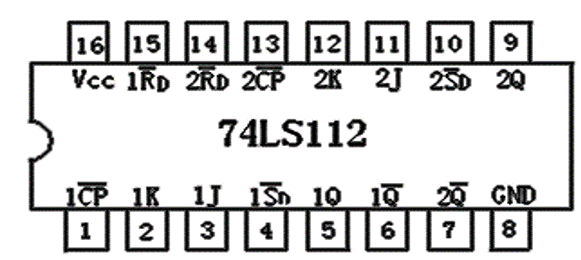
\includegraphics[scale = 0.6]{4.png}
                        \end{center}

                  \item [3.] D触发器  \\
                        在输入信号为单端的情况下,D触发器用起来最为方便,其状态方程为:$Q^{n+1} = D$\\
                        其输出状态的更新发生在CP脉冲的上升沿\\
                        由功能表可知D触发器输出状态与D端状态相同\\
                        \begin{itemize}

                              \item $CP$-时钟
                              \item $D$-输入端
                              \item $\overline{RD},\overline{SD}$-复位,重置端
                              \item $Q$,$\overline{Q}$输出端
                        \end{itemize}
                        \begin{center}
                              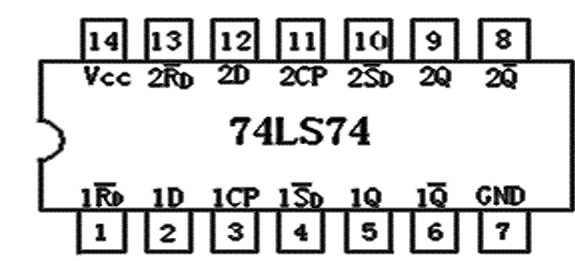
\includegraphics[scale = 0.6]{5.png}
                        \end{center}

            \end{itemize}
      \item 计算及仿真:  \\
            % \newpage



      \item  实验目的: \\

            \begin{itemize}
                  \item [1.]  了解时钟脉冲的触发作用。
                  \item [2.]  掌握基本RS、JK、D触发器的逻辑功能与使用方法。
                  \item [3.]  理解触发器所实现的状态转换功能。
            \end{itemize}

      \item  实验过程及数据分析:  \\
            \begin{itemize}
                  \item JK触发器测试电路  
                        \begin{center}
                              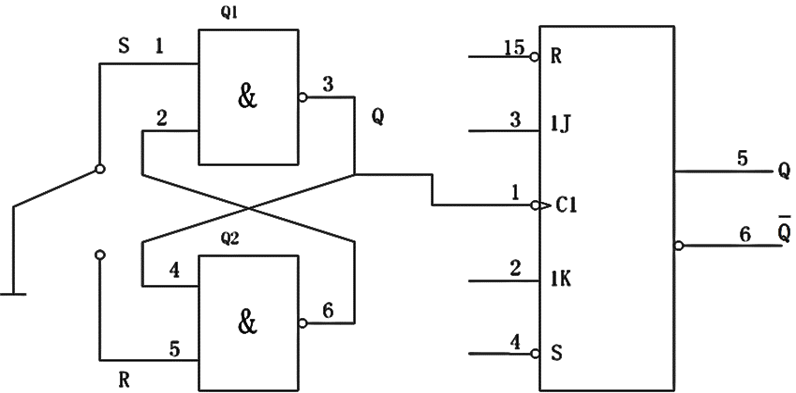
\includegraphics[scale = 0.6]{6.png}
                        \end{center}

                  \item JK触发器测试数据记录表  
                        \begin{center}
                              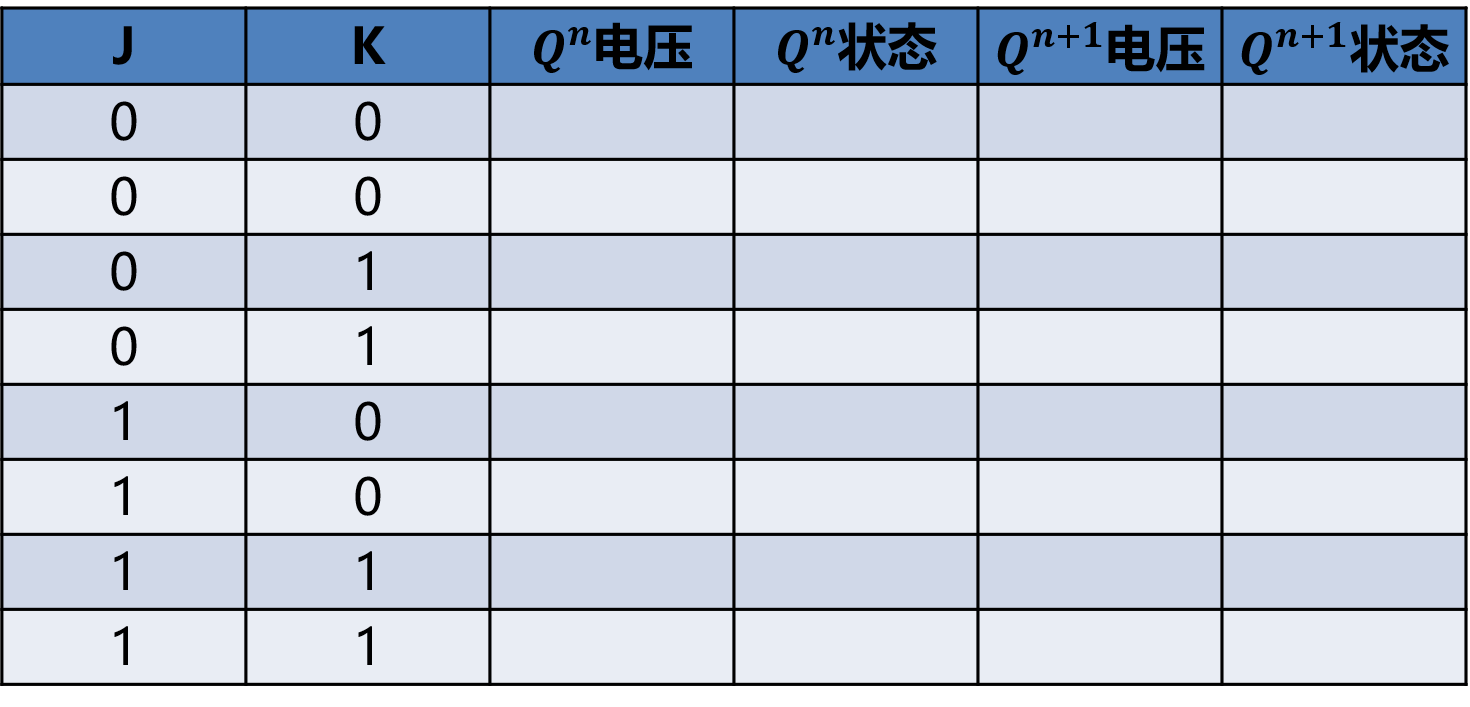
\includegraphics[scale = 0.6]{7.png}
                        \end{center}
                  \item D触发器测试电路  
                        \begin{center}
                              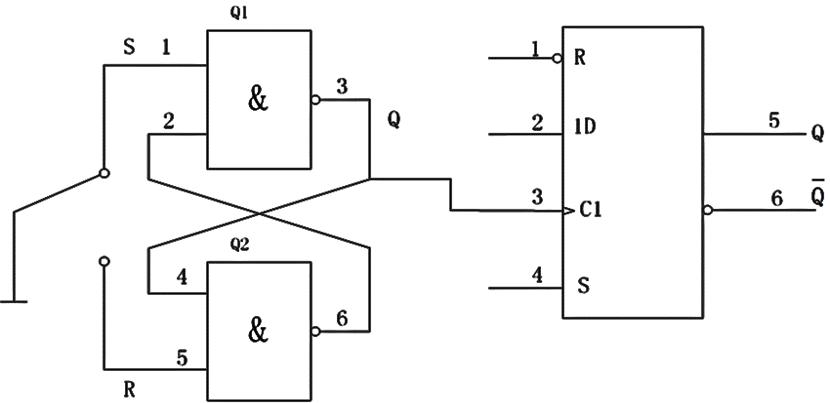
\includegraphics[scale = 0.6]{8.png}
                        \end{center}
                  \item D触发器测试数据记录表  
                        \begin{center}
                              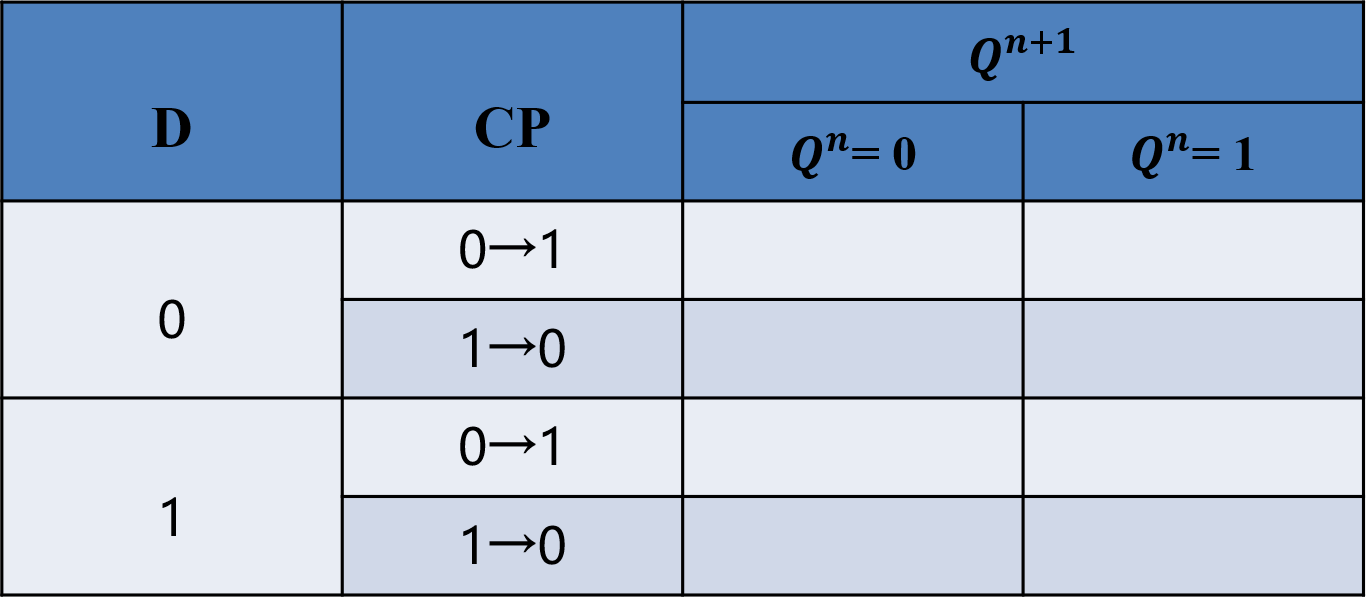
\includegraphics[scale = 0.6]{9.png}
                        \end{center}
            \end{itemize}
\end{enumerate}
\end{document}